\begin{figure}
  \begin{tabular}{ccccc}
    \begin{minipage}{0.2\hsize}
      \includegraphics[width=2.2cm]{../pic/Run78/KN_ana_NC170_2sigma/KNpi_MM_0.eps}
    \end{minipage}
    \begin{minipage}{0.2\hsize}
      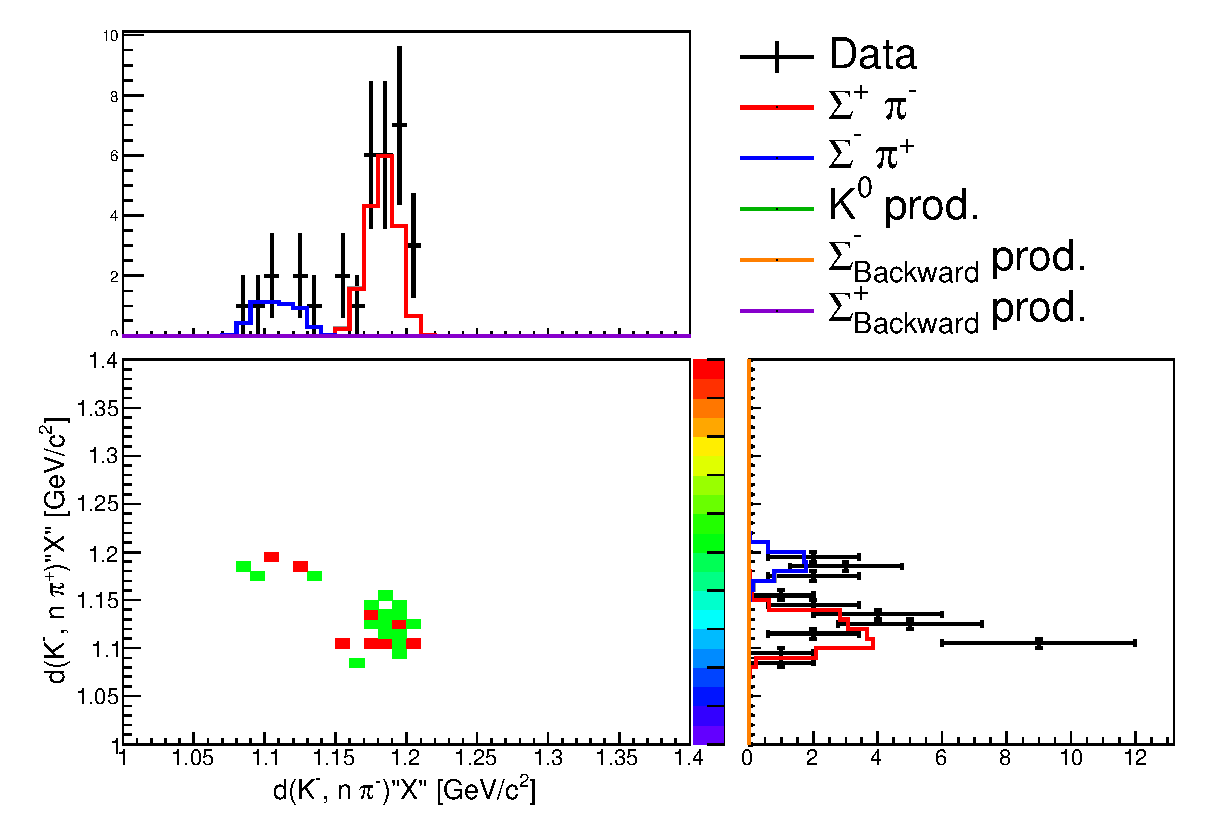
\includegraphics[width=2.2cm]{../pic/Run78/KN_ana_NC170_2sigma/KNpi_MM_1.eps}
    \end{minipage}
    \begin{minipage}{0.2\hsize}
      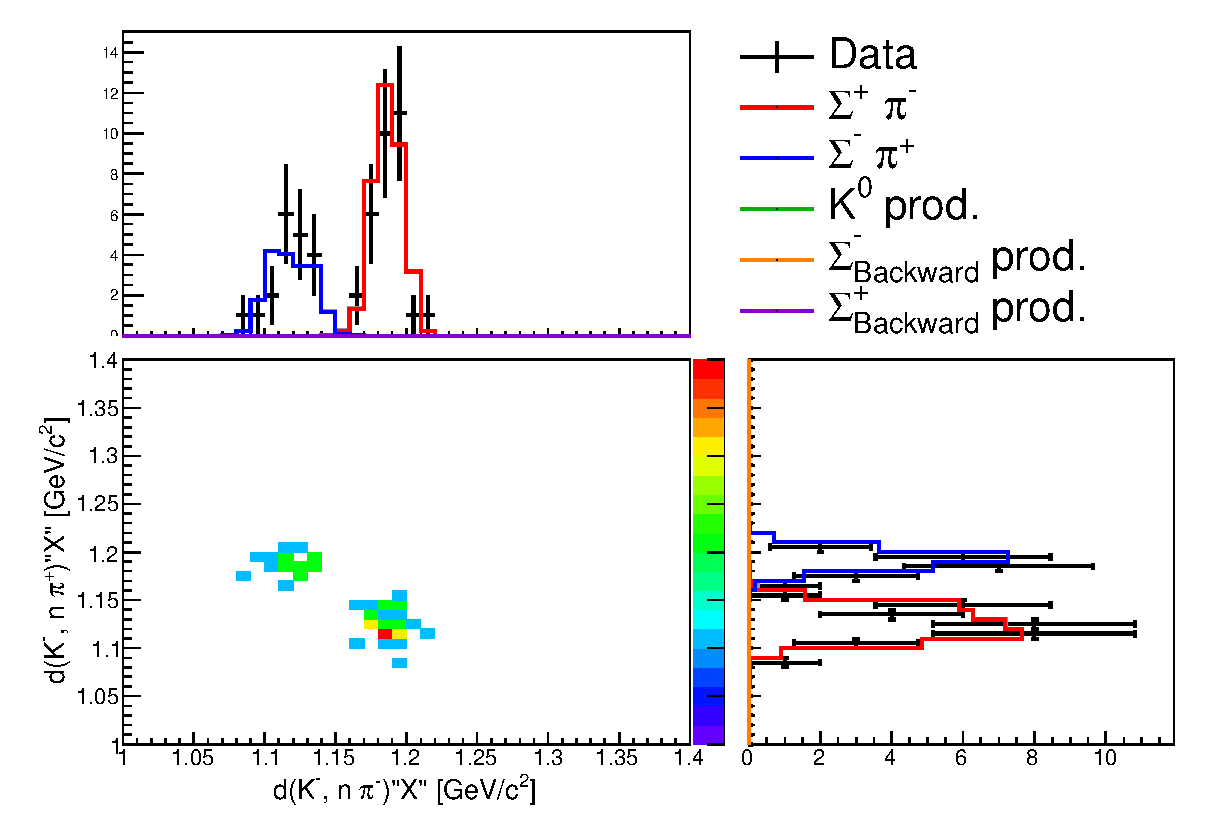
\includegraphics[width=2.2cm]{../pic/Run78/KN_ana_NC170_2sigma/KNpi_MM_2.eps}
    \end{minipage}
    \begin{minipage}{0.2\hsize}
      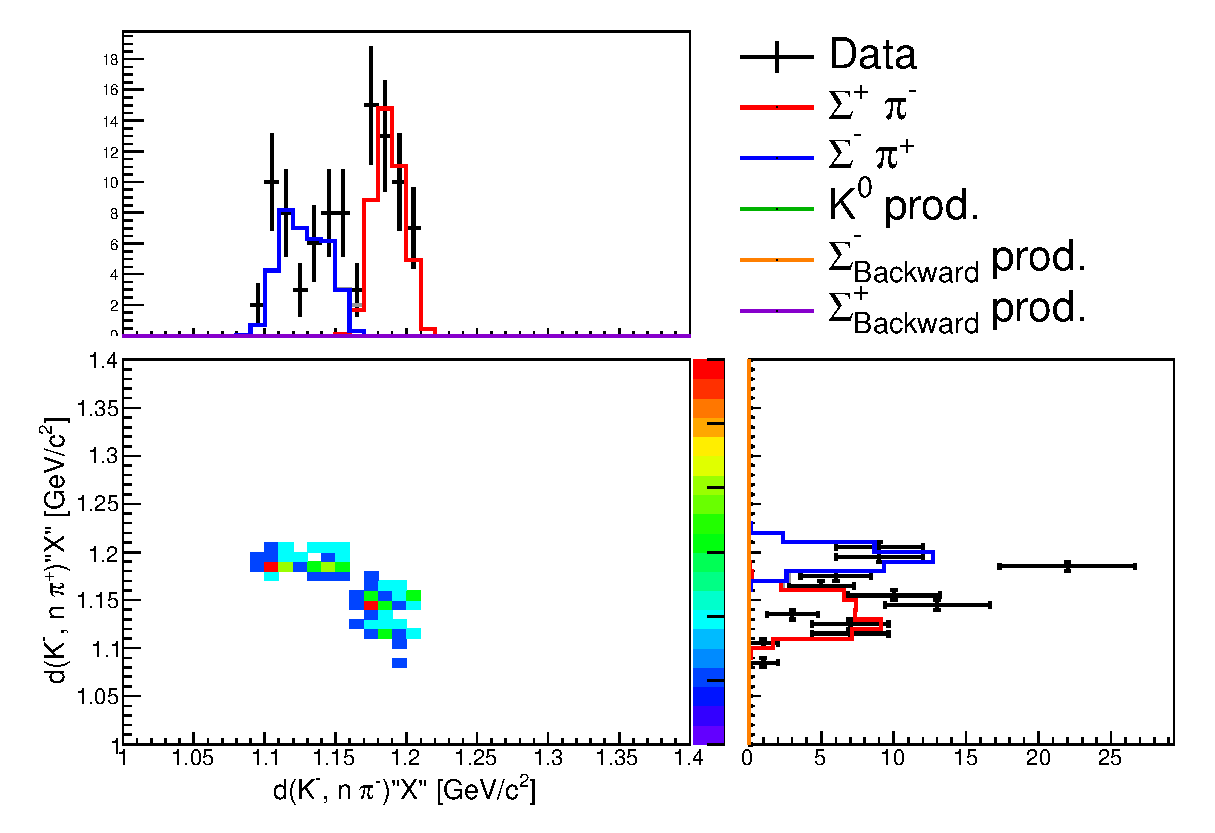
\includegraphics[width=2.2cm]{../pic/Run78/KN_ana_NC170_2sigma/KNpi_MM_3.eps}
    \end{minipage}
    \begin{minipage}{0.2\hsize}
      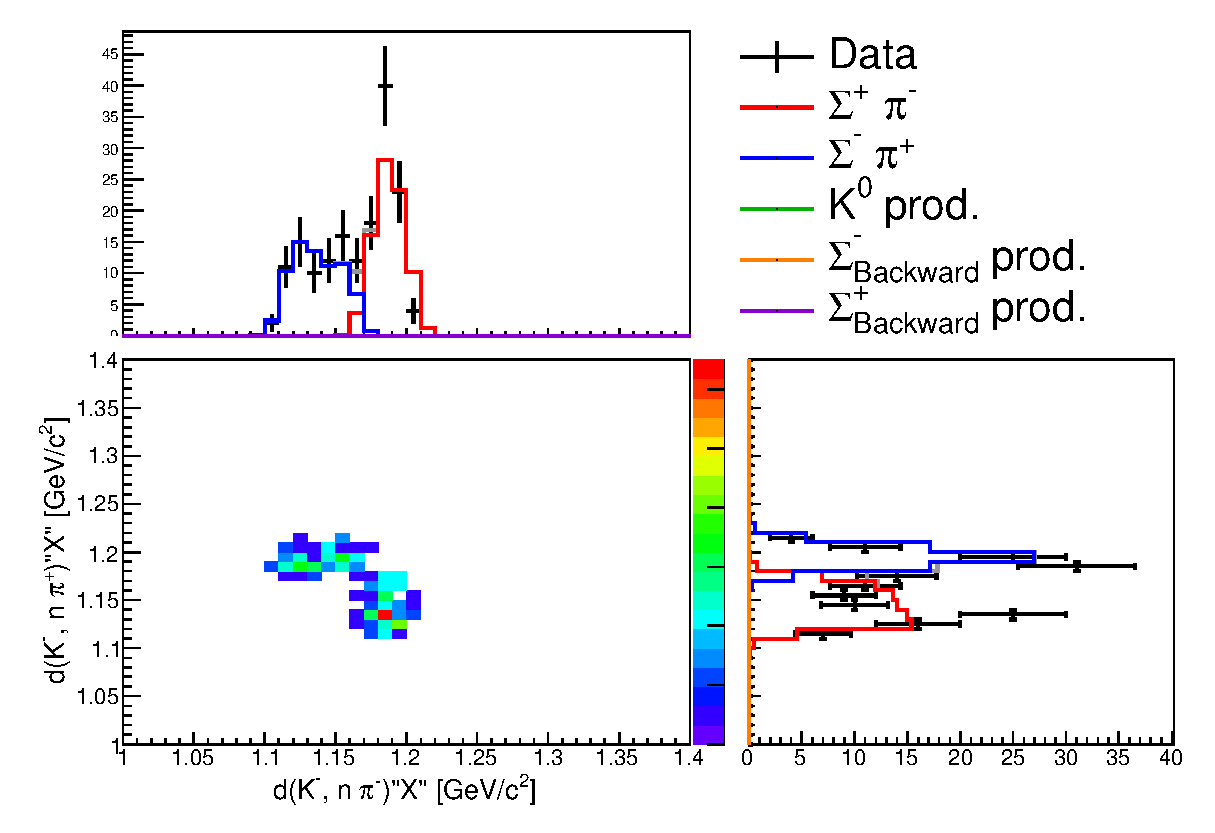
\includegraphics[width=2.2cm]{../pic/Run78/KN_ana_NC170_2sigma/KNpi_MM_4.eps}
    \end{minipage}
  \end{tabular}
  \begin{tabular}{ccccc}
    \begin{minipage}{0.2\hsize}
      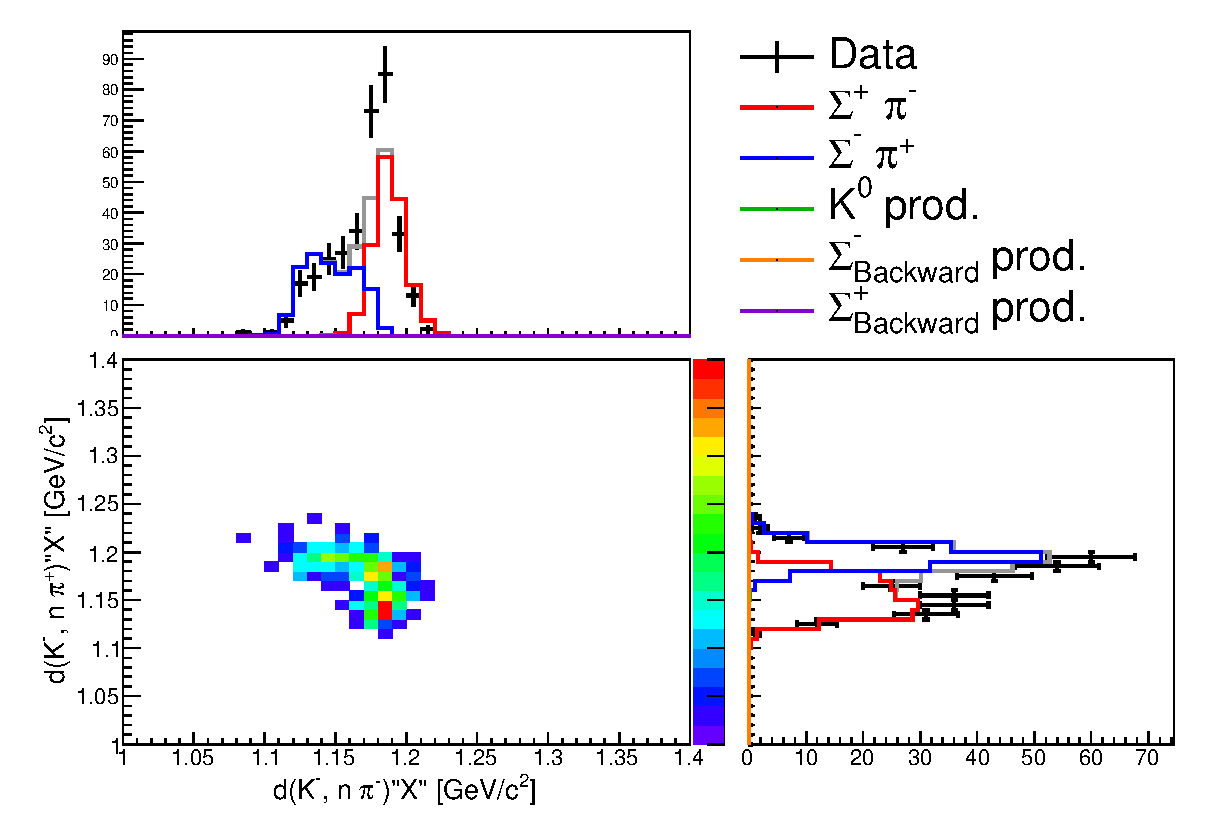
\includegraphics[width=2.2cm]{../pic/Run78/KN_ana_NC170_2sigma/KNpi_MM_5.eps}
    \end{minipage}
    \begin{minipage}{0.2\hsize}
      \includegraphics[width=2.2cm]{../pic/Run78/KN_ana_NC170_2sigma/KNpi_MM_6.eps}
    \end{minipage}
    \begin{minipage}{0.2\hsize}
      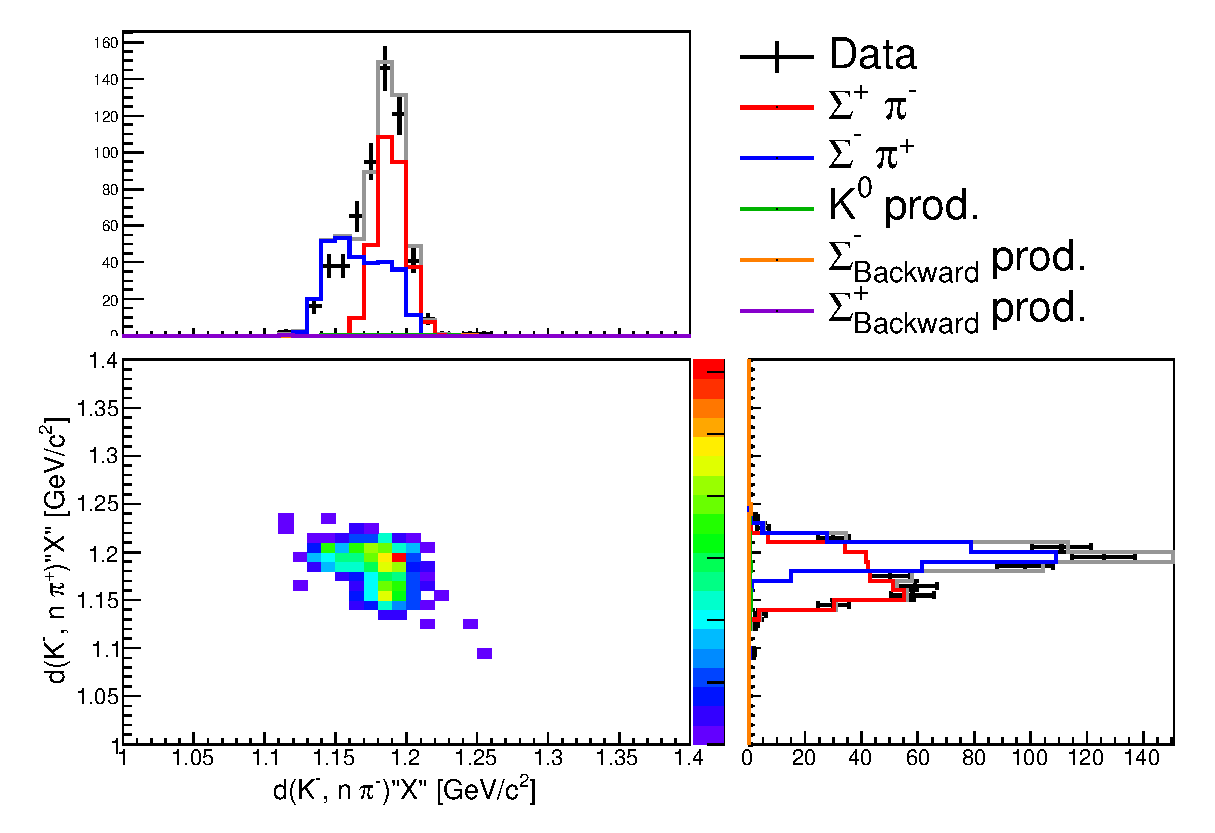
\includegraphics[width=2.2cm]{../pic/Run78/KN_ana_NC170_2sigma/KNpi_MM_7.eps}
    \end{minipage}
    \begin{minipage}{0.2\hsize}
      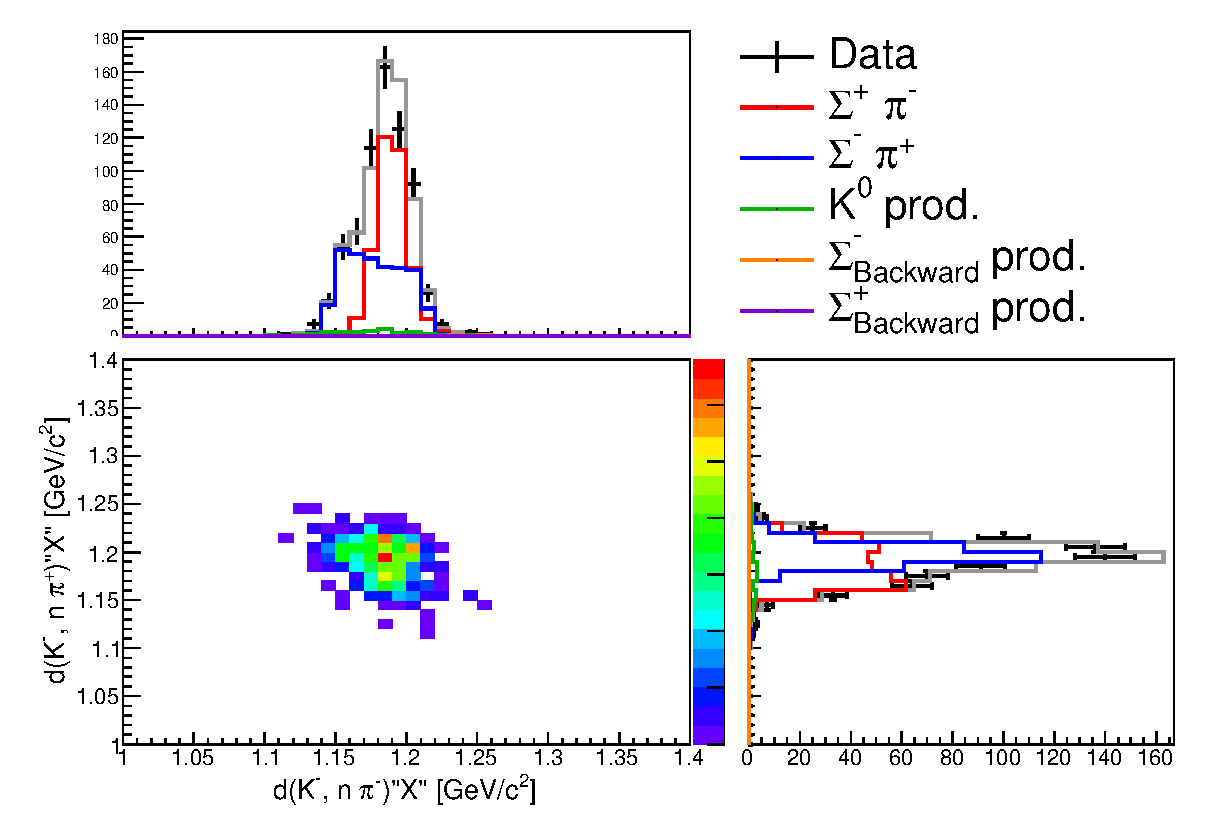
\includegraphics[width=2.2cm]{../pic/Run78/KN_ana_NC170_2sigma/KNpi_MM_8.eps}
    \end{minipage}
    \begin{minipage}{0.2\hsize}
      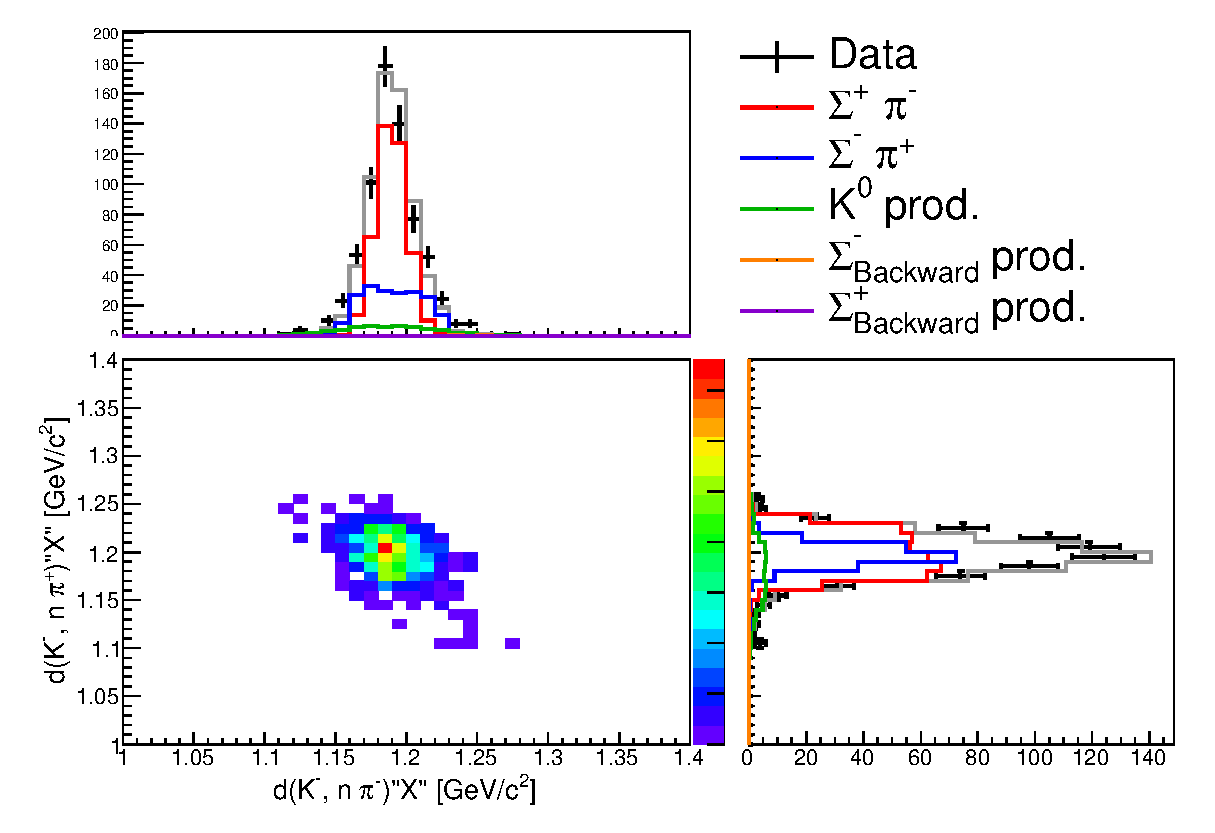
\includegraphics[width=2.2cm]{../pic/Run78/KN_ana_NC170_2sigma/KNpi_MM_9.eps}
    \end{minipage}
  \end{tabular}
  \begin{tabular}{ccccc}
    \begin{minipage}{0.2\hsize}
      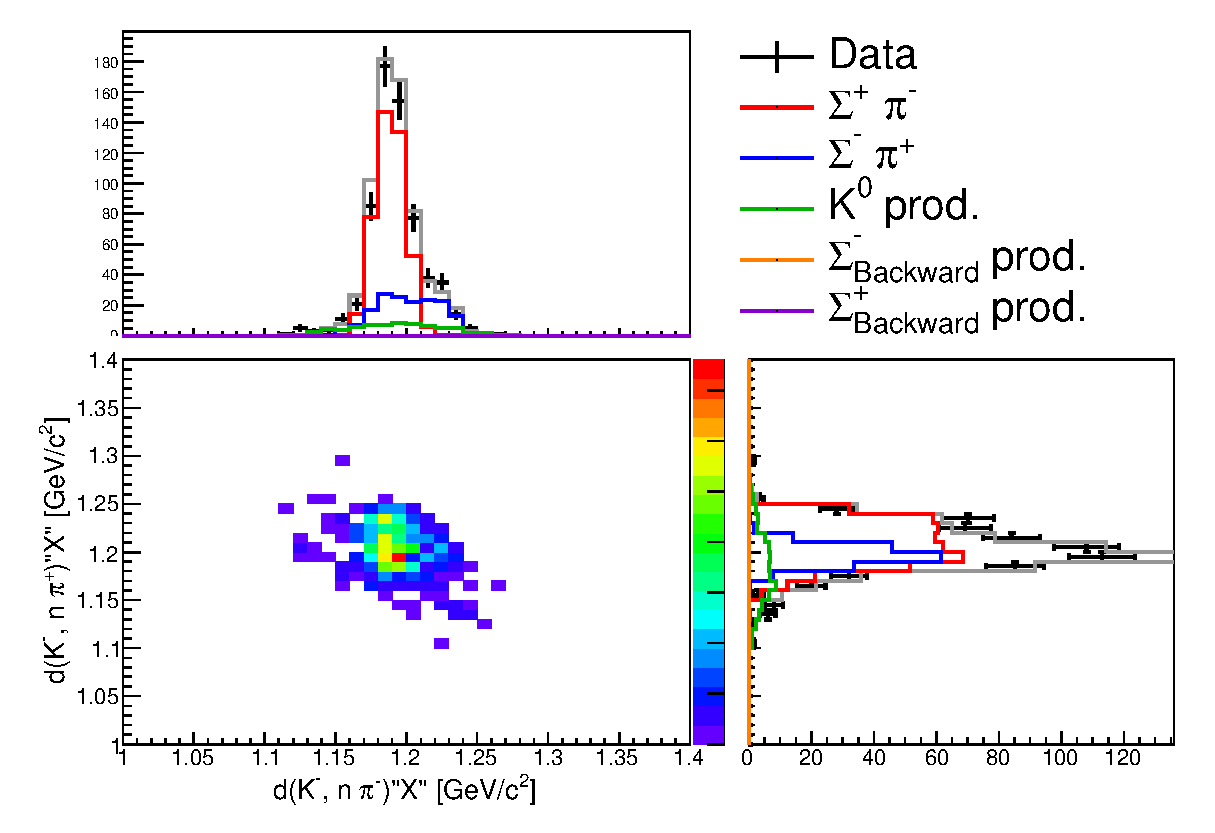
\includegraphics[width=2.2cm]{../pic/Run78/KN_ana_NC170_2sigma/KNpi_MM_10.eps}
    \end{minipage}
    \begin{minipage}{0.2\hsize}
      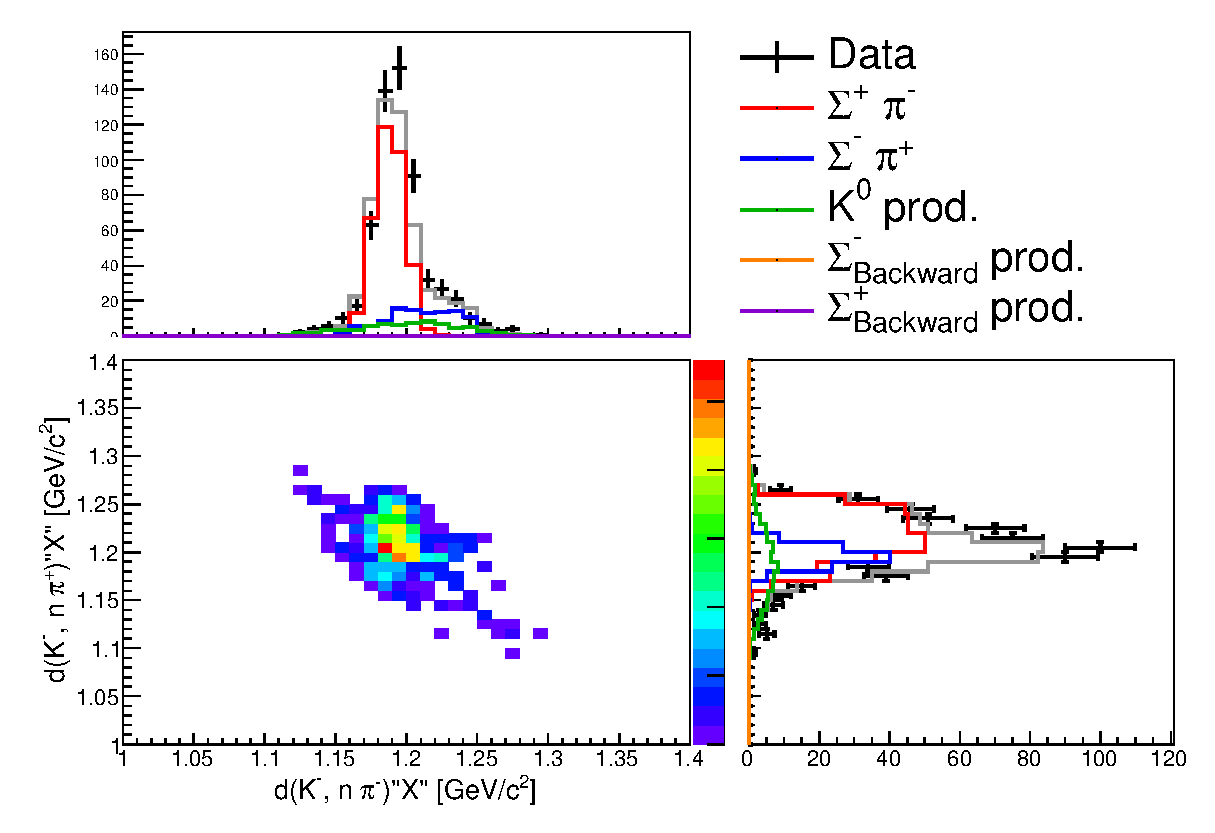
\includegraphics[width=2.2cm]{../pic/Run78/KN_ana_NC170_2sigma/KNpi_MM_11.eps}
    \end{minipage}
    \begin{minipage}{0.2\hsize}
      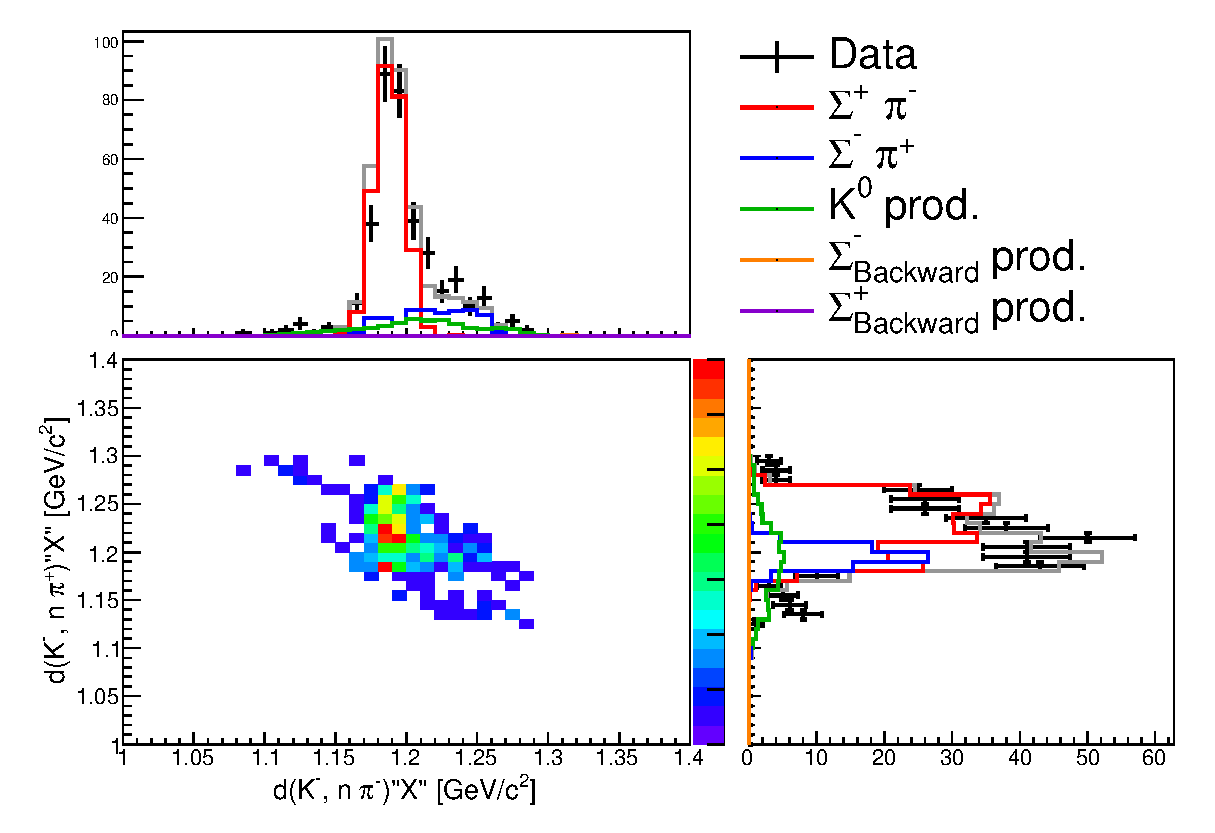
\includegraphics[width=2.2cm]{../pic/Run78/KN_ana_NC170_2sigma/KNpi_MM_12.eps}
    \end{minipage}
    \begin{minipage}{0.2\hsize}
      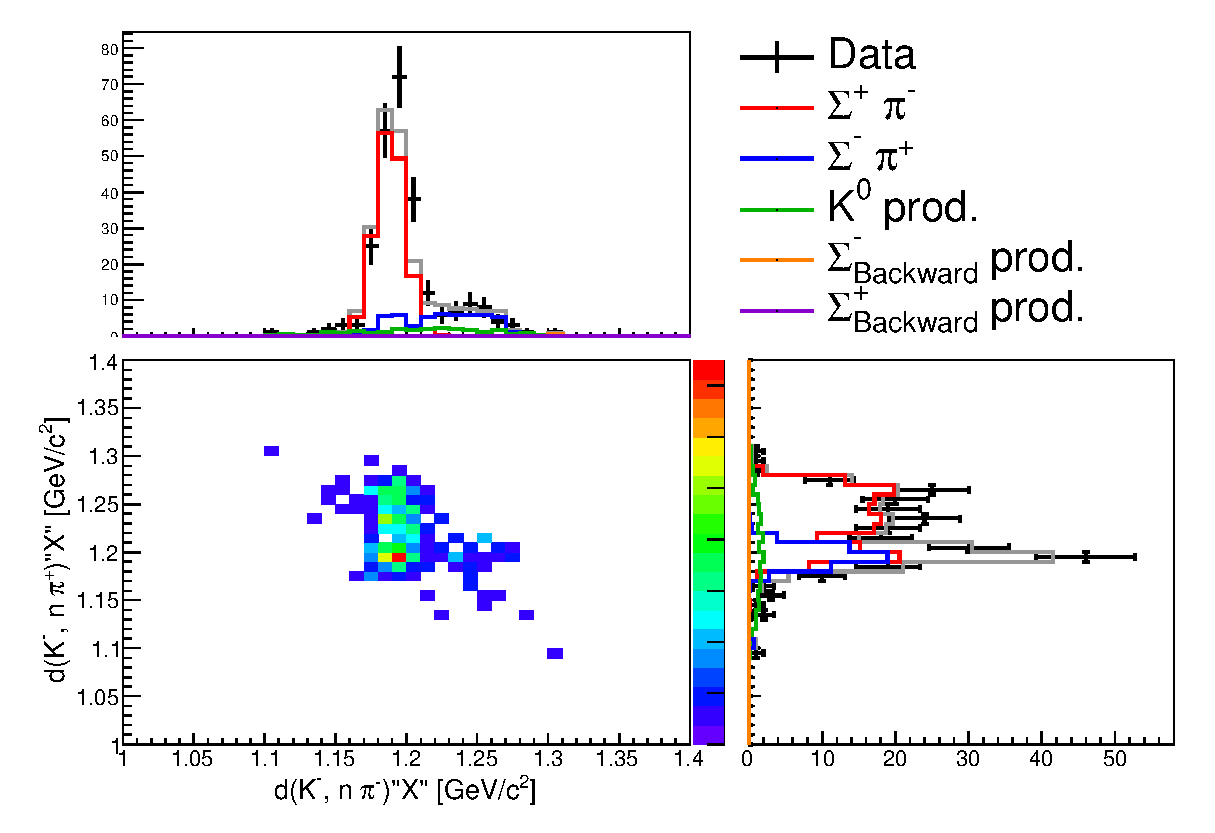
\includegraphics[width=2.2cm]{../pic/Run78/KN_ana_NC170_2sigma/KNpi_MM_13.eps}
    \end{minipage}
    \begin{minipage}{0.2\hsize}
      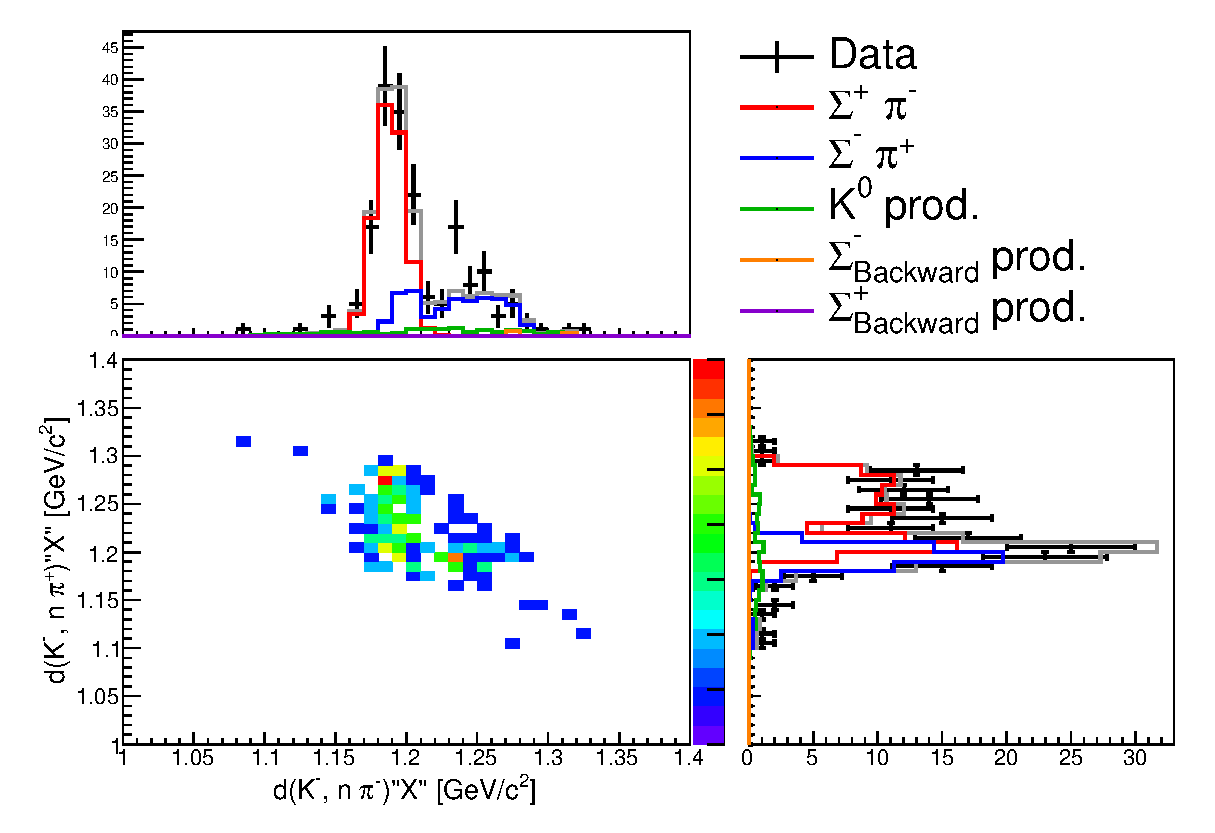
\includegraphics[width=2.2cm]{../pic/Run78/KN_ana_NC170_2sigma/KNpi_MM_14.eps}
    \end{minipage}
  \end{tabular}
  \begin{tabular}{ccccc}
    \begin{minipage}{0.2\hsize}
      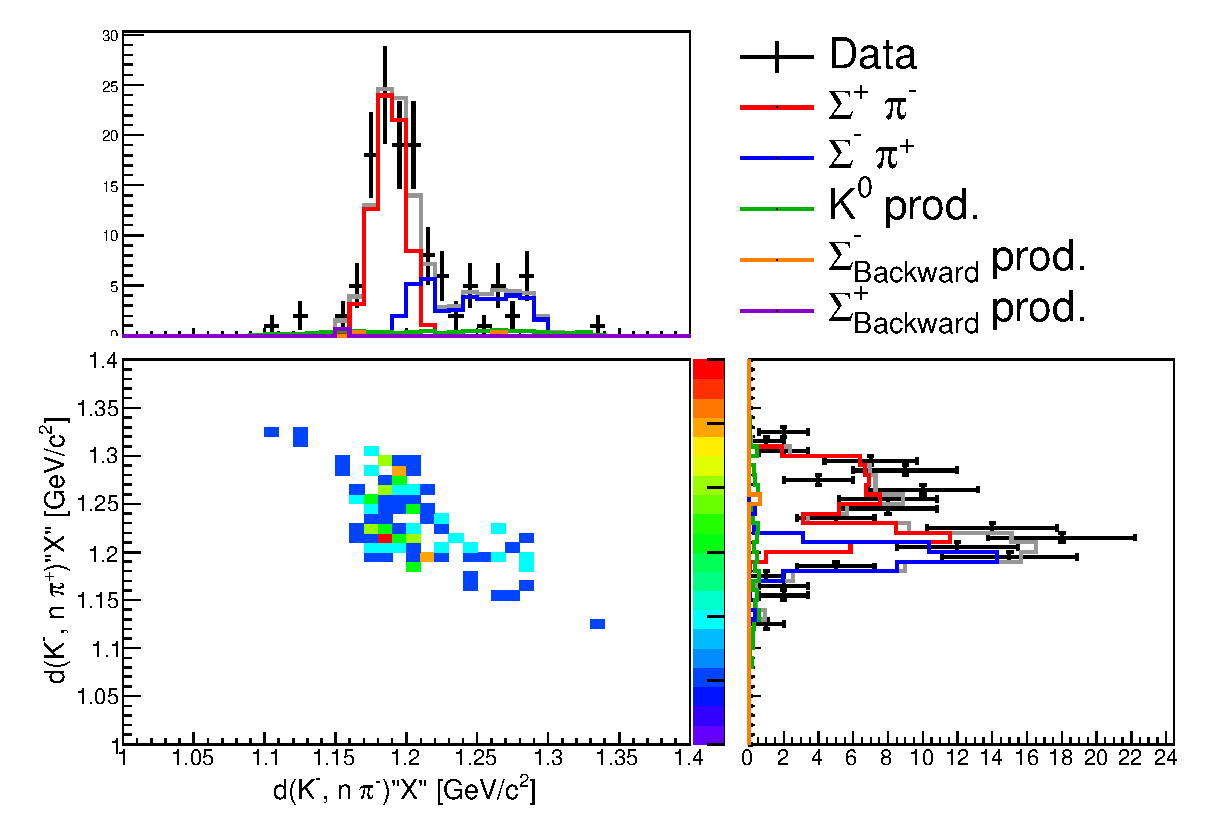
\includegraphics[width=2.2cm]{../pic/Run78/KN_ana_NC170_2sigma/KNpi_MM_15.eps}
    \end{minipage}
    \begin{minipage}{0.2\hsize}
      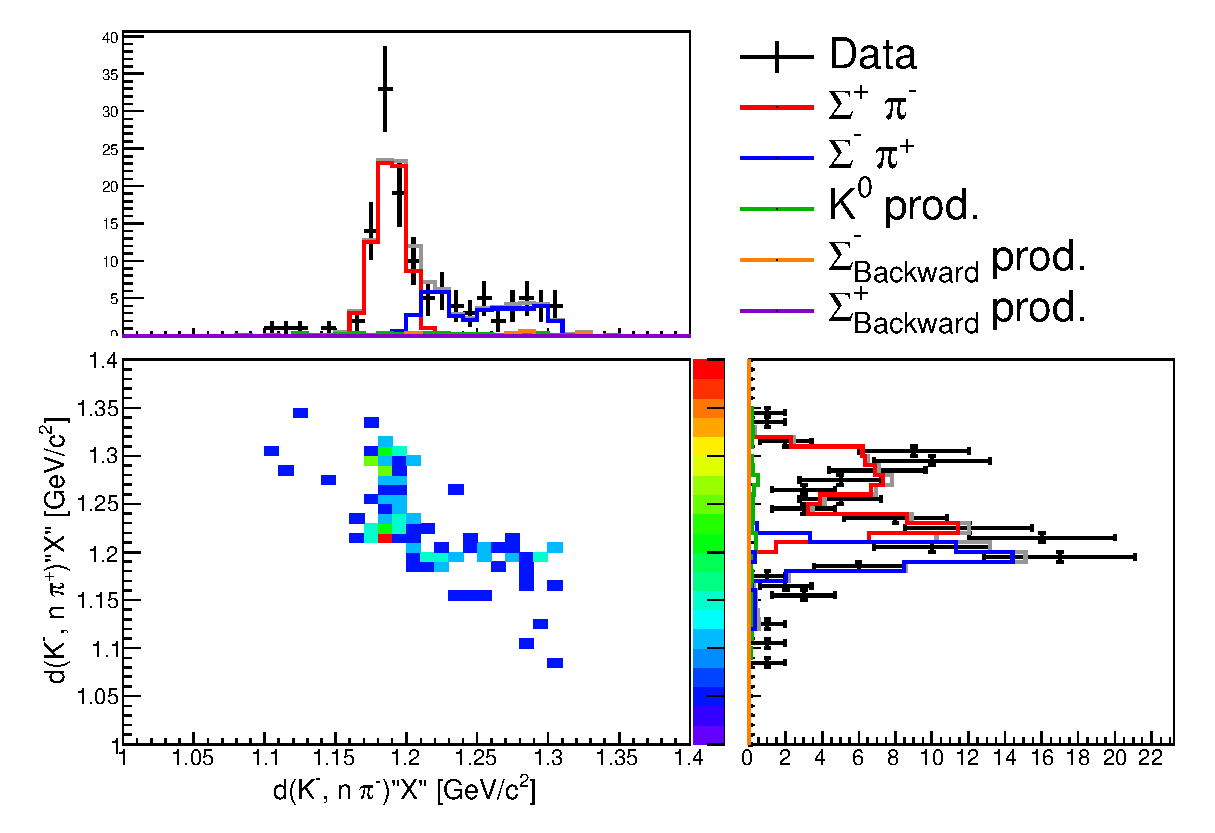
\includegraphics[width=2.2cm]{../pic/Run78/KN_ana_NC170_2sigma/KNpi_MM_16.eps}
    \end{minipage}
    \begin{minipage}{0.2\hsize}
      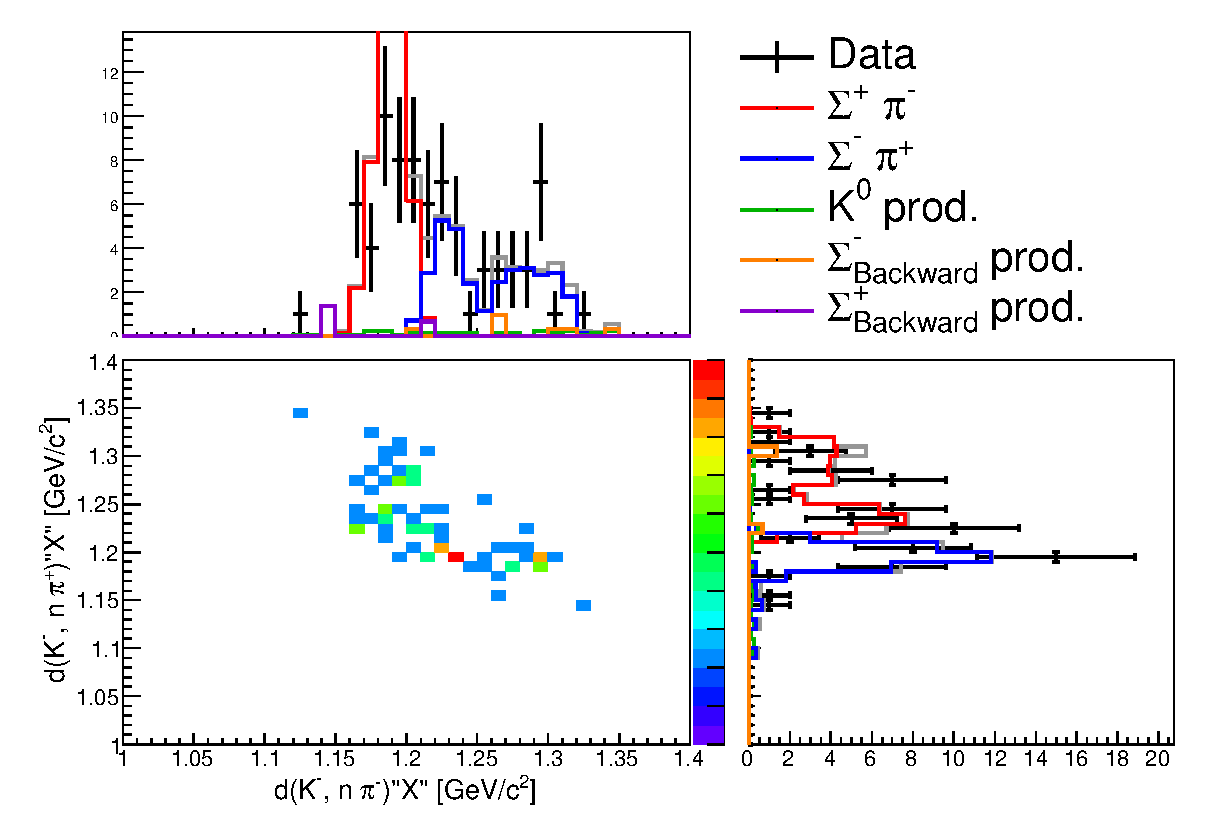
\includegraphics[width=2.2cm]{../pic/Run78/KN_ana_NC170_2sigma/KNpi_MM_17.eps}
    \end{minipage}
    \begin{minipage}{0.2\hsize}
      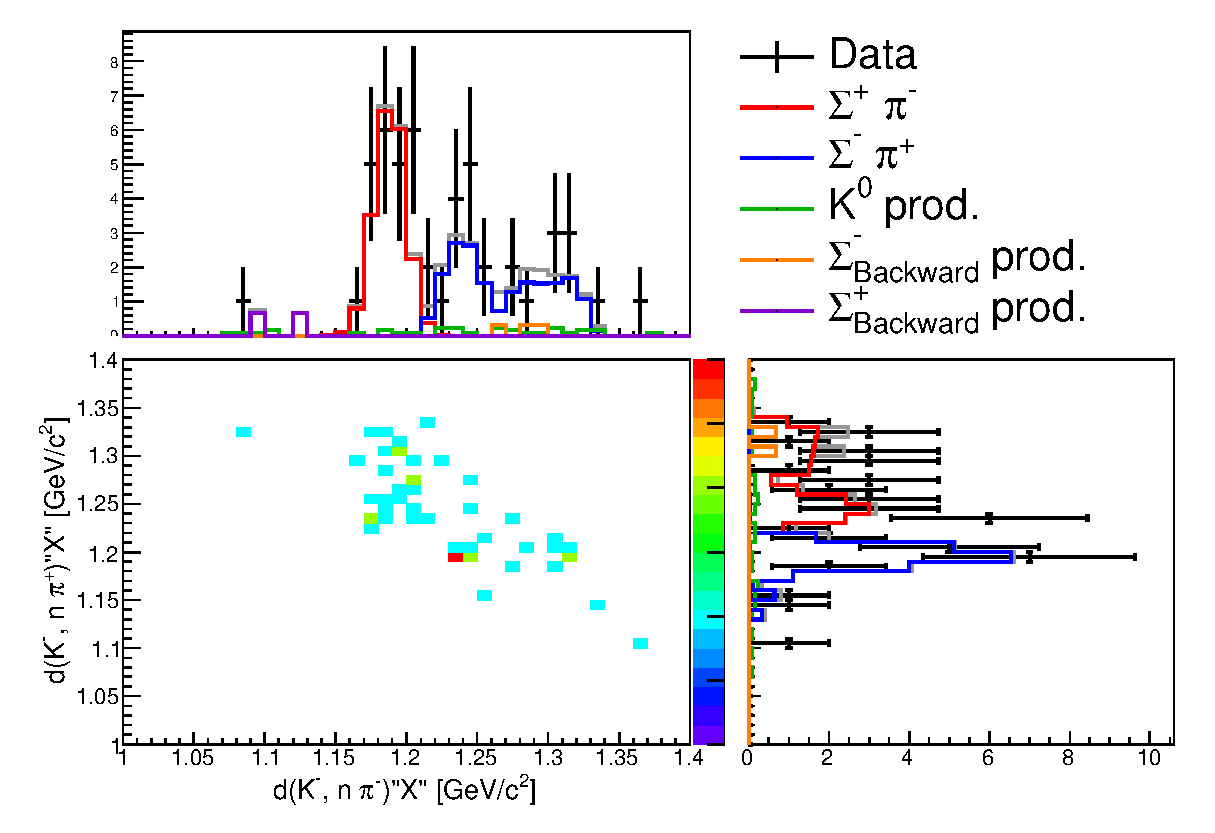
\includegraphics[width=2.2cm]{../pic/Run78/KN_ana_NC170_2sigma/KNpi_MM_18.eps}
    \end{minipage}
    \begin{minipage}{0.2\hsize}
      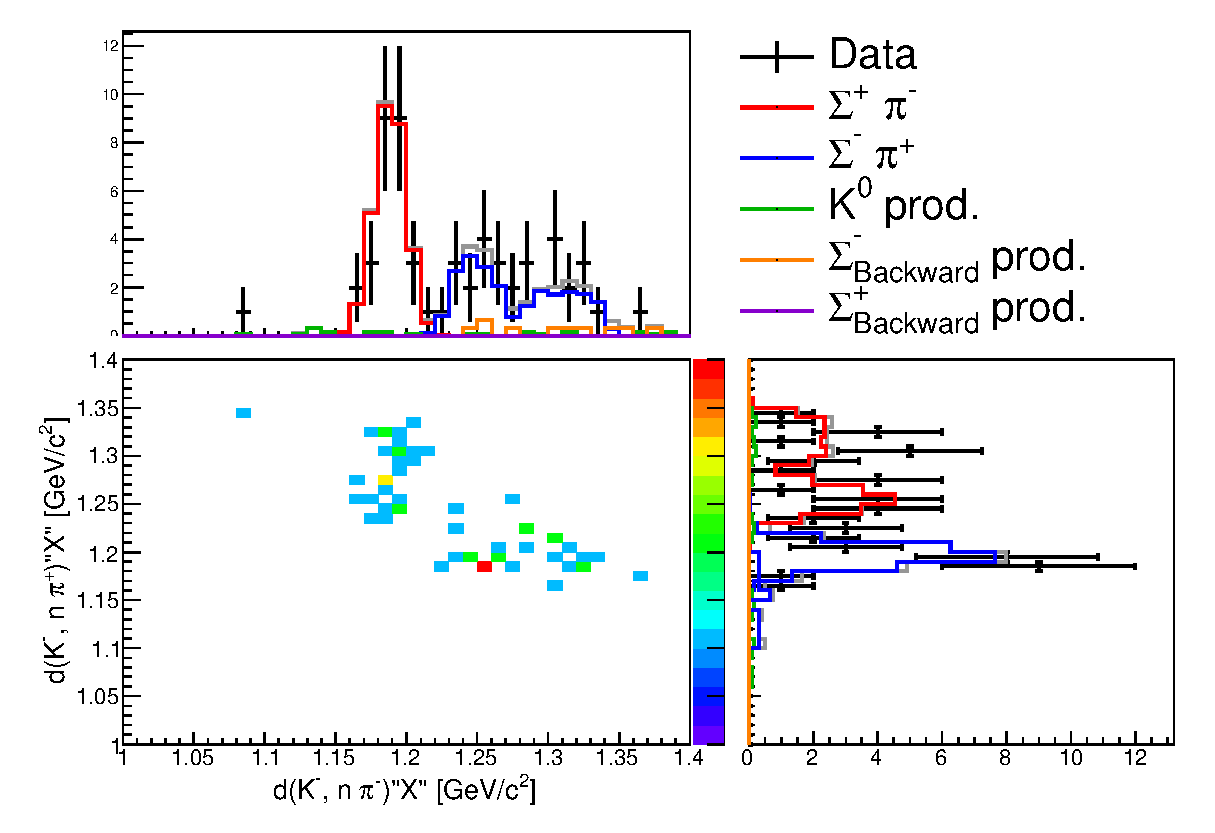
\includegraphics[width=2.2cm]{../pic/Run78/KN_ana_NC170_2sigma/KNpi_MM_19.eps}
    \end{minipage}
  \end{tabular}
  \begin{tabular}{ccccc}
    \begin{minipage}{0.2\hsize}
      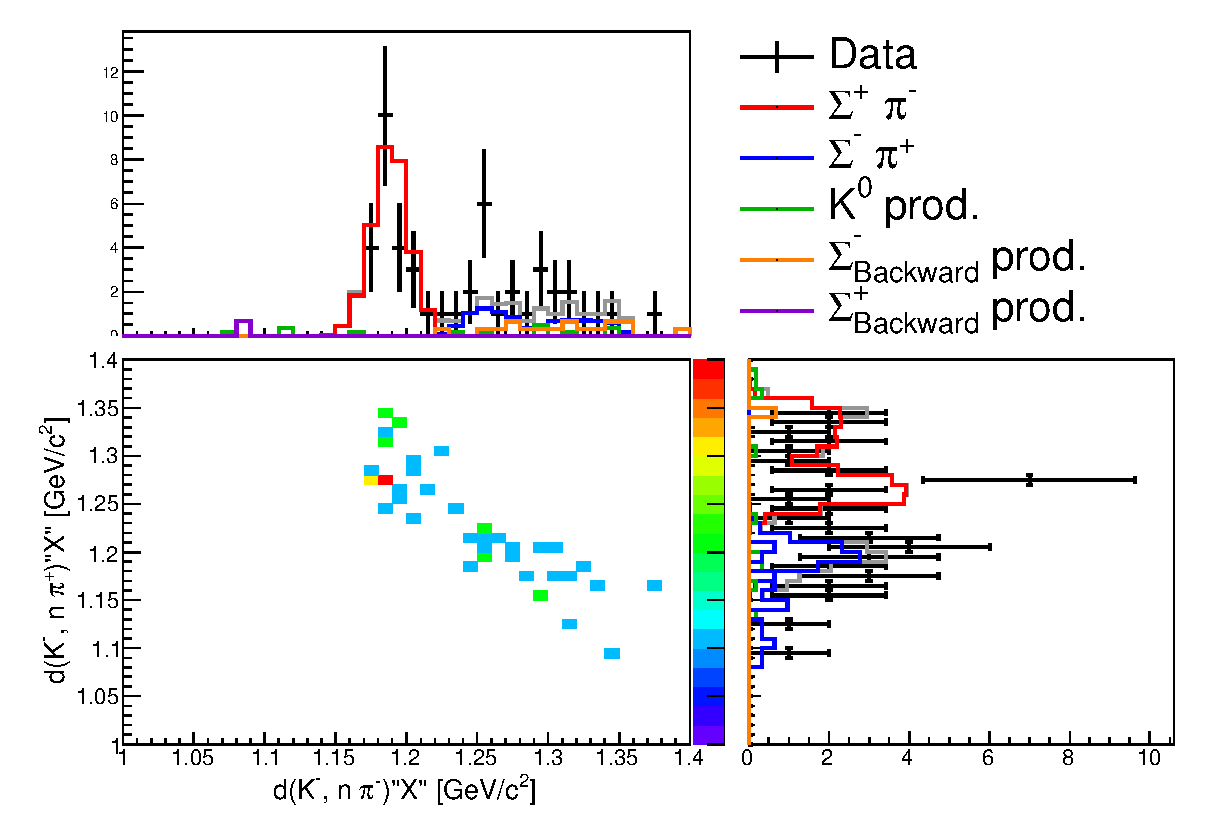
\includegraphics[width=2.2cm]{../pic/Run78/KN_ana_NC170_2sigma/KNpi_MM_20.eps}
    \end{minipage}
    \begin{minipage}{0.2\hsize}
      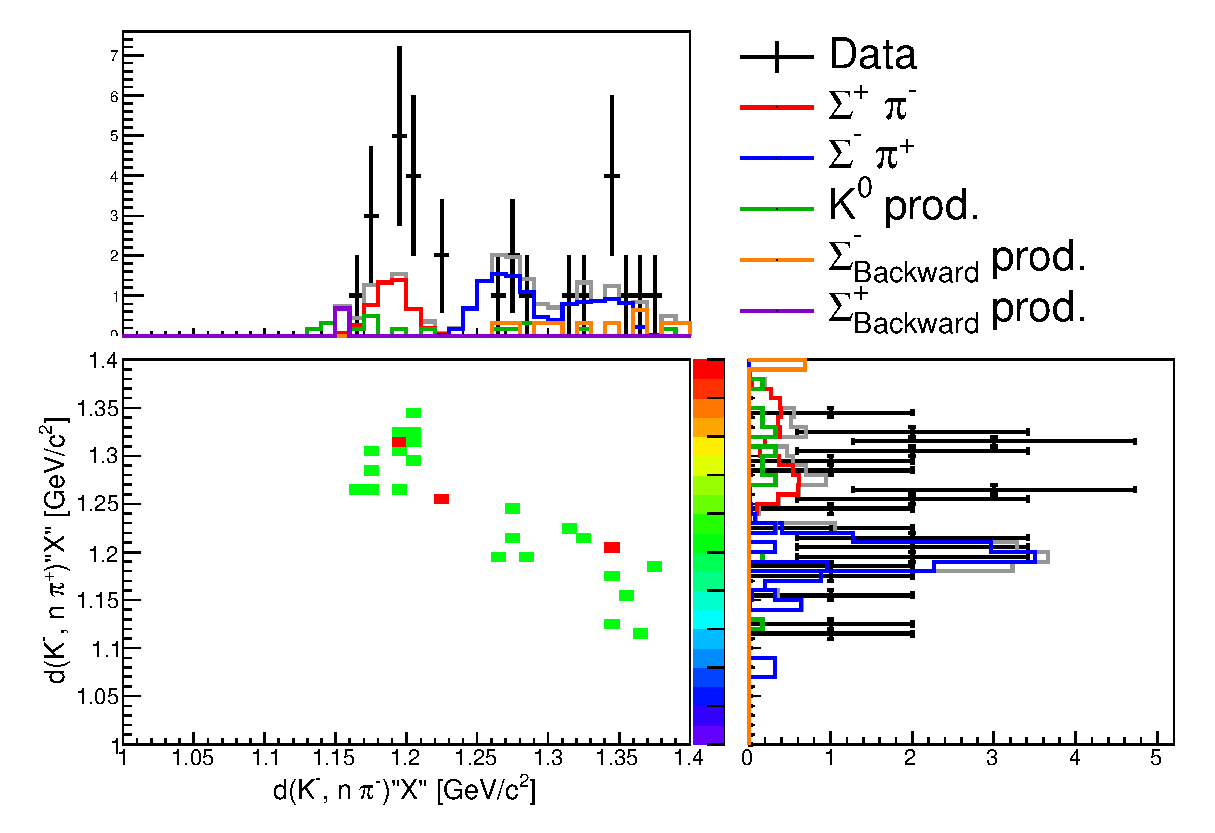
\includegraphics[width=2.2cm]{../pic/Run78/KN_ana_NC170_2sigma/KNpi_MM_21.eps}
    \end{minipage}
    \begin{minipage}{0.2\hsize}
      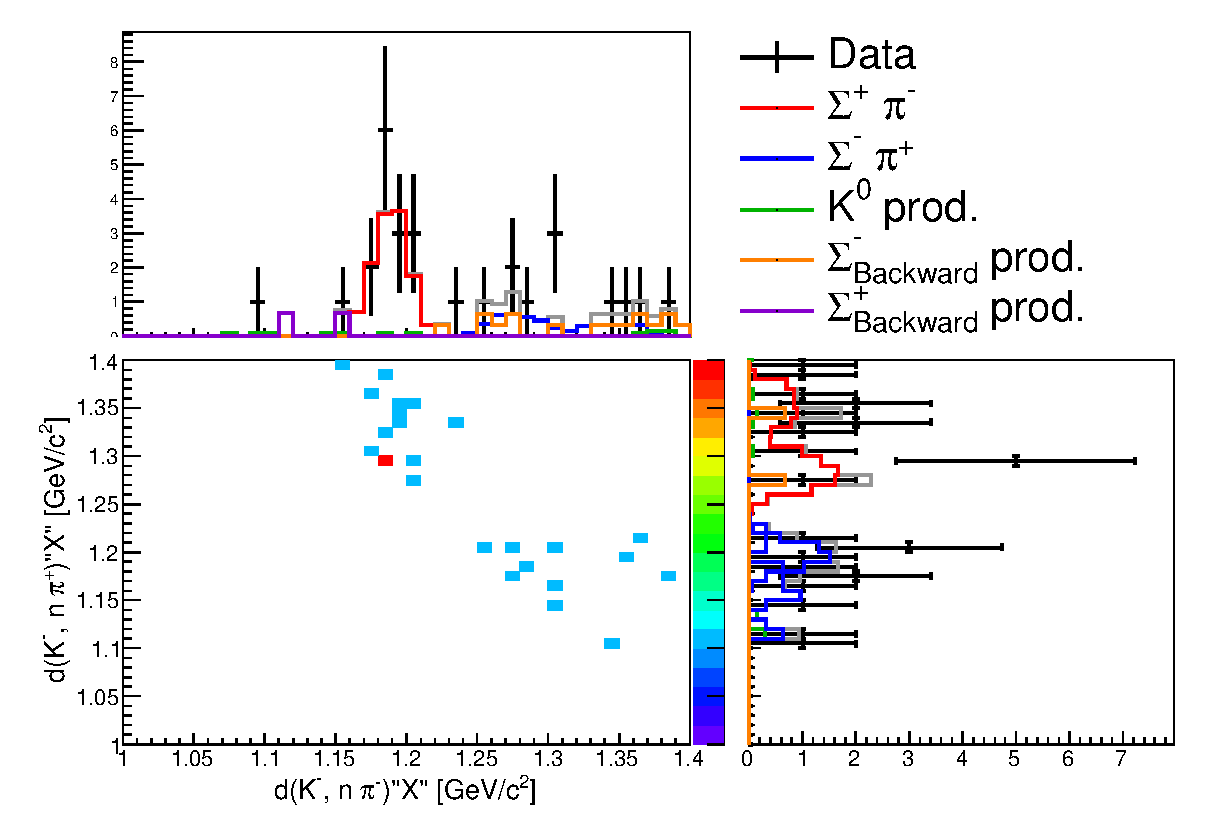
\includegraphics[width=2.2cm]{../pic/Run78/KN_ana_NC170_2sigma/KNpi_MM_22.eps}
    \end{minipage}
    \begin{minipage}{0.2\hsize}
      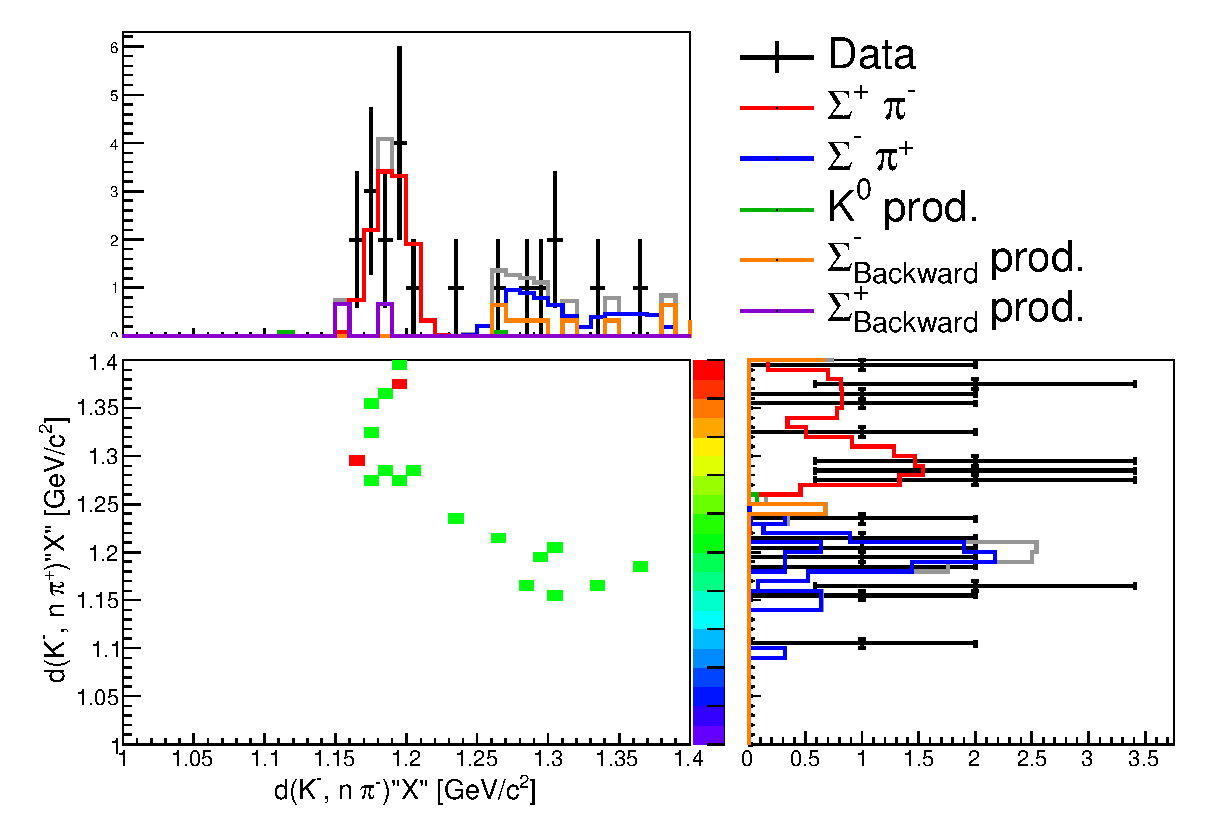
\includegraphics[width=2.2cm]{../pic/Run78/KN_ana_NC170_2sigma/KNpi_MM_23.eps}
    \end{minipage}
    \begin{minipage}{0.2\hsize}
      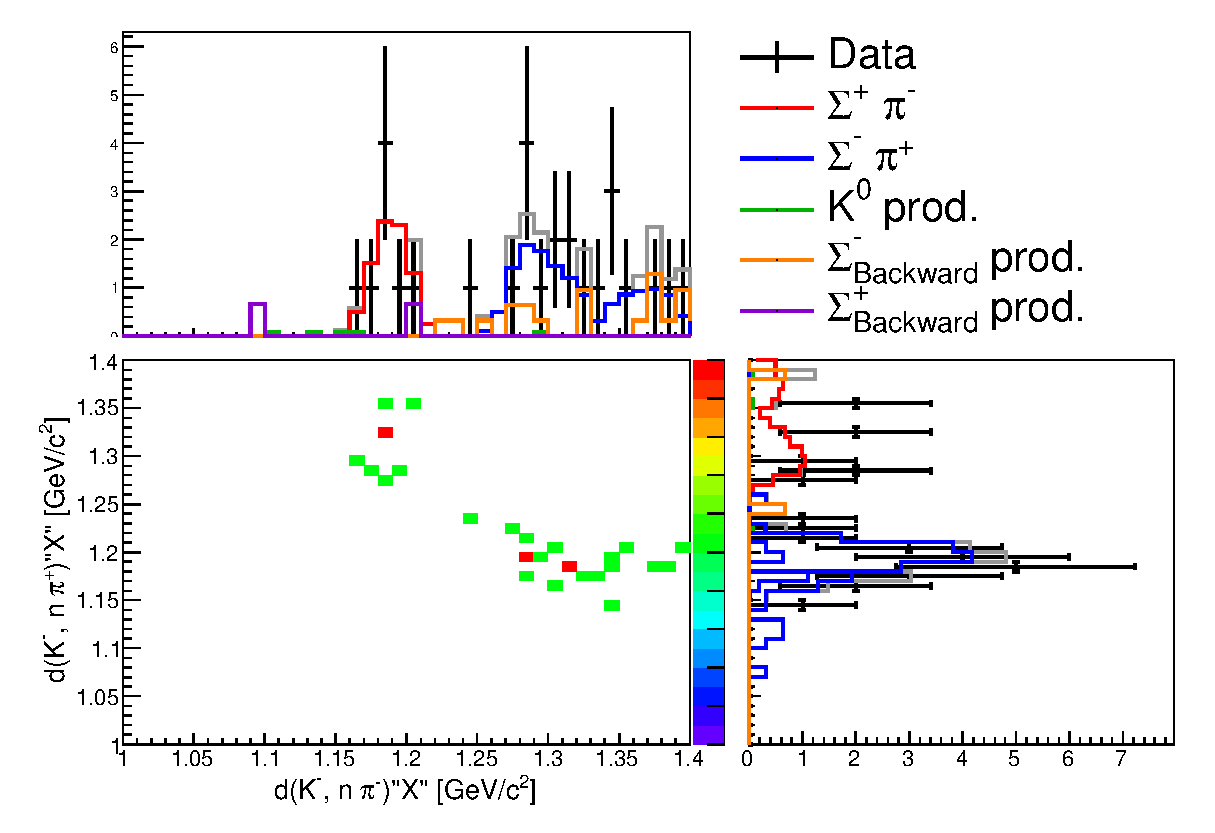
\includegraphics[width=2.2cm]{../pic/Run78/KN_ana_NC170_2sigma/KNpi_MM_24.eps}
    \end{minipage}
  \end{tabular}
  \label{fig:fit_KNpi_MM}
  \caption{
    These figures are presented separately for each bin of $d(K^-, n)$ for fitting to separate $\pi^- \Sigma^+$ and $\pi^+ \Sigma^-$ modes.
    The top left figure shows the lowest missing mass in the $1.35$-$1.36$GeV bin, with the next bin represented as one goes to the right.
    In other words, one row is shown for the 0.05GeV region.
  }
\end{figure}
